\documentclass{article}
\usepackage{graphicx} % Required for inserting images
\parindent=0pt
\usepackage{nameref}
\usepackage[utf8]{inputenc}
\usepackage{amsmath}
\usepackage{amsfonts}
\usepackage{amssymb}
\usepackage{amsthm}
\usepackage{array}
\usepackage{systeme}
\usepackage{titlesec}
\usepackage{xcolor}
\usepackage{mathtools}
\theoremstyle{definition}
\newtheorem*{theorem}{Theorem}
\newtheorem*{lemma}{Lemma}
\newtheorem*{corollary}{Corollary}
\newtheorem*{proposition}{Proposition}
\newtheorem*{claim}{Claim}
\newtheorem*{definition}{Definition}
\newtheorem*{example}{Example}
\newtheorem*{notation}{Notation}
\newtheorem*{conjecture}{Conjecture}
\theoremstyle{remark}
\newtheorem*{remark}{Remark}
\newcommand{\R}{\mathbb{R}}
\newcommand{\N}{\mathbb{N}}
\newcommand{\Nz}{\mathbb{N^*}}
\newcommand{\C}{\mathbb{C}}
\newcommand{\Q}{\mathbb{Q}}
\newcommand{\conj}[1]{\mkern 1.5mu\overline{\mkern-1.5mu#1\mkern-1.5mu}\mkern 1.5mu}
\newcommand{\tran}{^{\mkern-1.5mu\mathsf{T}}}
\DeclareMathOperator{\row}{row}
\DeclareMathOperator{\col}{col}
\DeclareMathOperator{\Span}{span}
\DeclareMathOperator{\rank}{rank}
\DeclareMathOperator{\Col}{Col}
\DeclareMathOperator{\dom}{dom}
\DeclareMathOperator{\im}{im}
\DeclareMathOperator{\tr}{tr}
\DeclareMathOperator{\id}{id}
\DeclareMathOperator{\sgn}{sgn}
\DeclareMathOperator{\adj}{adj}
\DeclareMathOperator{\Null}{Null}
\DeclareMathOperator{\dist}{dist}
\DeclareMathOperator{\proj}{proj}
\DeclareMathOperator{\E}{E}
\DeclareMathOperator{\var}{Var}
\DeclareMathOperator{\m}{m}
\DeclareMathOperator{\cov}{Cov}
\DeclareMathOperator{\diam}{\mathrm {diam}}
\DeclareMathOperator{\cl}{\mathrm {cl}}
\DeclareMathOperator{\interior}{int}
\DeclareMathOperator{\supp}{supp}
\DeclareMathOperator{\alint}{al\text{-}int}
\DeclareMathOperator{\aff}{aff}
\DeclareMathOperator{\co}{co}
\DeclareMathOperator{\cone}{cone}
\DeclareMathOperator{\p}{\mathbf p}
\newcommand\myfunc[5]{
  \begingroup
  \setlength\arraycolsep{0pt}
  #1\colon\begin{array}[t]{c >{{}}c<{{}} c}
             #2 & \to & #3 \\ #4 & \mapsto & #5 
          \end{array}%
  \endgroup}
\newcommand\PP[2]{P_{\mathcal #2\leftarrow \mathcal #1}}
\newcommand\M[2]{\mathcal M_{\mathcal #1; \mathcal #2}}
\newcommand\MM[1]{\mathcal M_{\mathcal #1}}
\newcommand \norm[1]{\left\lVert #1 \right\rVert}
\newcommand\inn [2]{\left\langle #1{,}#2\right\rangle}
\newcommand \unif {\overset{\text{unif}}\longrightarrow}
\newcommand \pw {\overset{\text{pw}}\longrightarrow}
\newcommand \as {\overset{\text{a.e.}}\longrightarrow}
\newcommand \pb {\overset{\text{pb}}\longrightarrow}
\newcommand \dis {\overset{\text{d}}\longrightarrow}
\newcommand \utimes {\underline{\times}}
\newcommand{\dott}{\,\begin{picture}(-1,1)(-1,-3)\circle*{3}\end{picture}\ }
\newcommand{\e}{\mathrm{e}}
\newcommand{\D}{\mathrm D}
\renewcommand{\i}{\mathrm{i}}
\newcommand{\B}{\mathrm B}
\renewcommand{\d}{\,\mathrm{d}}
\renewcommand{\epsilon}{\varepsilon}
\renewcommand{\emptyset}{\varnothing}
\usepackage[left=2cm,right=2cm,top=2cm,bottom=2cm]{geometry}
\usepackage{enumitem}

\title{Continuous Optimization: Homework 1}
\author{Edoardo Gargiulo, Matteo Martellini, Marco Bares, Adrian Fluder, Andreas Jean T Caeyman}
\date{30 September 2026}

\begin{document}

\maketitle
\section*{Question 1}
Recall that we defined $\phi\colon \R\to \R$ by $$\phi(z)=\begin{cases}
    0, &\text{ if }z\leq -1\\
    \frac 12 (1+z)^2, &\text{ if }-1<z<0\\
    \frac 12 +z, &\text{ if }z\geq 0
\end{cases},$$  $f\colon \mathcal E\to \R$  by $$f(\theta)=\sum\limits_{i=1}^m  \phi\left( s_i\inn{{\tilde{x}_i}}{\theta} \right)=\sum\limits_{i=1}^m  \phi\left( \inn{{s_i\tilde{x}_i}}{\theta} \right)$$
and $f_{\lambda}\colon \mathcal E\to \R$ (with $\lambda>0)$ by
$$
f_\lambda(\theta)=f(\theta)+\frac{\lambda}{2}\norm{\theta}^2.
$$
We will show that $f_\lambda$ is $\lambda$-strongly convex, i.e. that $f$ is convex. Since the composition of a convex functions with a linear function is again convex and so is the sum of convex functions, we will be done if we can show that $\phi$ is convex.
Elementary calculus shows that $\phi\in \mathcal C^1(\R) $ with
$$\phi'(z)=\begin{cases}
    0, &\text{ if }z\leq -1\\
     1+z, &\text{ if }-1<z<0\\
    1, &\text{ if }z\geq 0
\end{cases};$$
in particular, $\phi'$ is non-decreasing, whence $\phi$ is convex.
We have shown that $f_\lambda$ is $\lambda$-strongly convex, whence, by theorem 4.28, $f_\lambda$ admits one and only one point of global minimum.
The set of global minimizers of a $C^1$ convex function coincides with the set of critical points by corollary 4.23; it follows $f_\lambda$ has exactly one critical point. 

\section*{Question 2}
For this and the following questions, we  fix $\lambda=0.005$.
Recall form question 1 that $\phi\in \mathrm C^1(\R)$, whence $\D \phi (z)[v]=\phi'(z)\cdot v$, for each $z,v\in \R$.
Since the differential operator $\D(\cdot)$ is linear and the differential of a linear map at a fixed point is the linear map itself, we have that
\begin{align*}
  \D f(\theta)[v] &= \sum_{i=1}^m  \D \left( \phi\circ \inn{s_i\tilde{x_i}}{\cdot} \right)(\theta)[v]\\
  &= \sum_{i=1}^m  \D \phi(\inn{s_i\tilde{x_i}}{\theta}) 
\left[ \D (\inn{s_i\tilde{x_i}}{\cdot})(\theta)[v] \right]\\
&= \sum_{i=1}^m   \phi'(\inn{s_i\tilde{x_i}}{\theta}) \cdot
 \D (\inn{s_i\tilde{x_i}}{\cdot})(\theta)[v] \\
&=  \sum_{i=1}^m   \phi'(\inn{s_i\tilde{x_i}}{\theta}) \cdot
  \inn{s_i\tilde{x_i}}{v}\\
  &=\inn{\sum_{i=1}^m  \phi'(s_i\inn{\tilde{x_i}}{\theta})s_i\tilde{x_i}}{v}.
\end{align*}
Consider now the function $g\colon \mathcal E\to \R$ defined by $g(\theta)=\norm \theta^2$. We claim that $g$ is continuously differentiable with $\D g(\theta)[v]=\inn {2\theta}{v}$, for each $\theta,v\in \mathcal E$. To wit, fix  $\theta,v\in \mathcal E$ and compute
\begin{align*}
\frac{g(\theta+v)-g(\theta)-\inn{2\theta}{v}}{\norm v} &= \frac{\norm{\theta+v}^2-\norm{\theta}^2-\inn{2\theta}{v}}{\norm v}\\
&=\frac{\norm \theta^2 +2\inn {\theta}{v}+\norm v^2-\norm \theta^2-\inn{2\theta}{v}}{\norm v}\\
&=\norm v;
\end{align*}
it follows that $\lim\limits_{v\to 0}\frac{g(\theta+v)-g(\theta)-\inn{2\theta}{v}}{\norm v}=0$, which proves our claim (the continuity of the differential is obvious from its analytic expression).

Since $f_\lambda=f+\frac \lambda 2 g$, by linearity of the differential we have that, for arbitrary $\theta\in \mathcal E$,
$$
\D f_\lambda(\theta)[v]=\inn{\sum_{i=1}^m   \phi'(s_i\inn{\tilde{x_i}}{\theta})s_i\tilde{x_i}+\lambda\theta}{v}, \text{ for each }v\in \mathcal E,
$$
whence, by definition of the gradient, $\nabla f_\lambda(\theta)=\lambda\theta+\sum_{i=1}^m   \phi'(s_i\inn{\tilde{x_i}}{\theta})s_i\tilde{x_i}$, where the expression for $\phi'$ is given explicitly in the previous question.

To verify the numerical agreement, we used \texttt{np.allclose} on the outputs $a$ and $b$ of the loop-based and vectorized implementations, respectively. This function ensures that for all elements:
$$
\lvert a - b \rvert \leq \text{atol} + \text{rtol} \times \lvert b \rvert
$$
where we set both \texttt{atol} and \texttt{rtol} to $10^{-5}$.
\vspace{1em}

In terms of algorithmic complexity, both versions share the same order of magnitude regarding the number of operations, which fails to capture the overhead of the Python interpreter and the inner optimizations of vectorized code. The key difference is that the vectorized implementation delegates all operations to highly optimized under-the-hood C routines in NumPy. 

To appreciate the performance gap, we simply measured the execution time required to evaluate both the function and its gradient across all images in the dataset. Specifically, evaluating both $f_\lambda$ and $\nabla f_\lambda$ with a random initialization of $\theta$ required $0.1614$ seconds for the loop-based version, whereas the vectorized implementation took only $0.1008$ seconds. This represents a computing time reduction of approximately $37.5\%$, confirming the efficiency of bypassing Python loops in favor of NumPy's contiguous memory layouts and compiled under-the-hood operations.

\section*{Question 3}
\label{Q3}
To verify the numerical implementation of the gradient, we perform a first-order Taylor test. Let $\theta$ be a chosen point in the parameter space and let $v$ be a unit vector, i.e.,
\[
\|v\| = 1.
\]

For a range of step sizes
\[
t \in \{10^{-8}, \ldots, 10^0\},
\]
we consider the Taylor remainder
\[
E(t)
=
\left|
f_\lambda(\theta + tv)
-
f_\lambda(\theta)
-
t\left\langle v,\nabla f_\lambda(\theta)\right\rangle
\right|.
\]

If the gradient implementation is correct, the first-order Taylor expansion gives
\[
f_\lambda(\theta + tv)
=
f_\lambda(\theta)
+
t\left\langle v,\nabla f_\lambda(\theta)\right\rangle
+
\mathcal{O}(t^2).
\]

Hence,
\[
E(t) = \mathcal{O}(t^2).
\]

In particular, for sufficiently small $t$, we expect approximately
\[
E(t) \approx C t^2,
\]
for some constant $C>0$. Taking logarithms gives
\[
\log E(t)
\approx
\log C + 2\log t.
\]

Therefore, in a log-log plot of $E(t)$ against $t$, the approximately linear portion of the curve should have slope close to $2$.



\begin{figure}
    \centering
    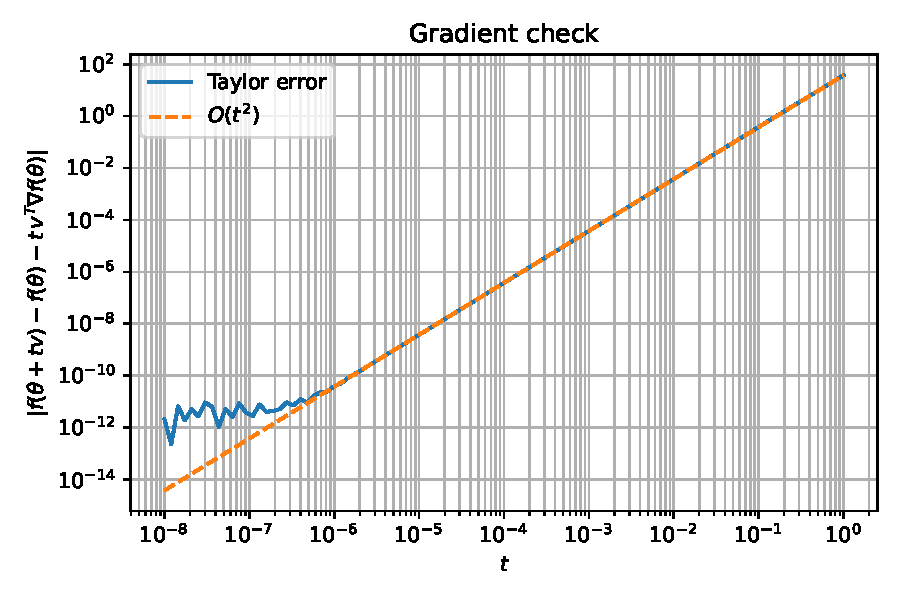
\includegraphics[width=0.5\linewidth]{results/q3_gradient_check.pdf}
    \caption{Gradient check showing second-order decay of the Taylor remainder.}    \label{fig:gradient_check}
\end{figure}


The numerical experiment conducted in \ref{fig:gradient_check} indeed shows an approximately straight region with slope close to $2$. This agrees with the expected second-order decay of the Taylor remainder and therefore supports the numerical correctness of the implemented gradient.



For very small values of \(t\), the Taylor error no longer follows the expected quadratic behavior. This can be explained by floating-point round-off and, in particular, by catastrophic cancellation. Indeed, \(f_\lambda(\theta+tv)\) and \(f_\lambda(\theta)\) become nearly equal as \(t\) decreases. Subtracting these nearly equal floating-point numbers may cause a significant loss of relative precision. Consequently, for sufficiently small \(t\), numerical round-off errors dominate the theoretical \(\mathcal{O}(t^2)\) Taylor remainder.


The observed slope does not constitute a formal proof that the gradient implementation is correct. The test is performed only for one particular point $\theta$, one direction $v$, and finitely many values of $t$. An incorrect implementation could, in principle, still pass such a finite numerical test. The gradient check should therefore be interpreted as strong numerical evidence rather than as a mathematical proof.

\section*{Question 4}
\label{Q4}

We implement gradient descent with a fixed constant step size according to
\[
\theta_{k+1}
=
\theta_k-\alpha \nabla f_\lambda(\theta_k),
\qquad k\geq 0,
\]
where $\lambda=0.005$ and $\nabla f_\lambda$ is the gradient derived in Question 2. The initial point $\theta_0\in\mathbb{R}^d$ is sampled from a standard Gaussian distribution using a fixed random seed, so that all experiments use the same reproducible initialization.

At every iteration $k\geq 0$, including the initial point, we record the objective value $f_\lambda(\theta_k)$ and the gradient norm $\norm{\nabla f_\lambda(\theta_k)}$. The algorithm terminates when $\norm{\nabla f_\lambda(\theta_k)} \leq 10^{-3}\norm{\nabla f_\lambda(\theta_0)}$, or when the time limit of three minutes is reached. The corresponding stopping condition is also recorded.

To choose the constant step size $\alpha$, we performed a grid search over
\[
\alpha\in
\left\{
10^{-2},10^{-3},10^{-4},10^{-5},10^{-6},10^{-7}
\right\}.
\]
on the training set from mnist\_train\_test.mat.
Each candidate was run from the same initial point $\theta_0$ and with the same three-minute time limit. We selected the step size yielding the smallest final objective value $f_\lambda(\theta_{\mathrm{final}})$ on average across seeds 0, 1 and 2. The results are summarized below in Table~\ref{tab:q4_grid_search}.

\begin{table}[h]
\centering
\caption{Grid search over step size $\alpha$: final objective value, number of iterations, and stopping reason (mean $\pm$ std over 3 seeds).}
\label{tab:q4_grid_search}
\begin{tabular}{c|c|c|c}
$\alpha$ &
Final $f_\lambda$ &
Iterations &
Stopping reason
\\ \hline
$10^{-2}$ & $3519.5277 \pm 3484.7116$ & $156.7 \pm 11.2$ & gradient tolerance \\
$10^{-3}$ & $309.9754 \pm 309.8209$ & $169.0 \pm 25.2$ & gradient tolerance \\
$10^{-4}$ & $47.2178 \pm 36.1661$ & $772.3 \pm 670.1$ & gradient tolerance \\
$10^{-5}$ & $54.3816 \pm 19.9279$ & $5592.3 \pm 3437.5$ & gradient tol. (2/3), time limit (1/3) \\
$10^{-6}$ & $284.2377 \pm 39.3962$ & $8840.0 \pm 516.1$ & time limit \\
$10^{-7}$ & $1801.6259 \pm 580.6248$ & $8877.7 \pm 495.3$ & time limit
\end{tabular}
\end{table}

Among the tested values, $\alpha=10^{-4}$ achieves the smallest final objective value on average. Moreover, unlike the smaller step sizes in general, it reaches the chosen gradient tolerance before the three-minute time limit. We therefore choose
\[
\boxed{\alpha=10^{-4}}
\]
for the final run. This illustrates a fundamental trade-off: larger step sizes terminate more quickly but yield larger final objective values, whereas smaller step sizes make insufficient progress within the available time budget.

\section*{Question 5}

We run the fixed-step gradient descent method from Question 4 on the training set from mnist\_train\_test.mat, starting from the same initial point $\theta_{0}$. Figure~\ref{fig:q5_convergence} shows the objective value $f_\lambda(\theta_k)$ and the gradient norm $\norm{\nabla f_\lambda(\theta_k)}$ as functions of the iteration number $k$.

\begin{figure}[h]
    \centering
    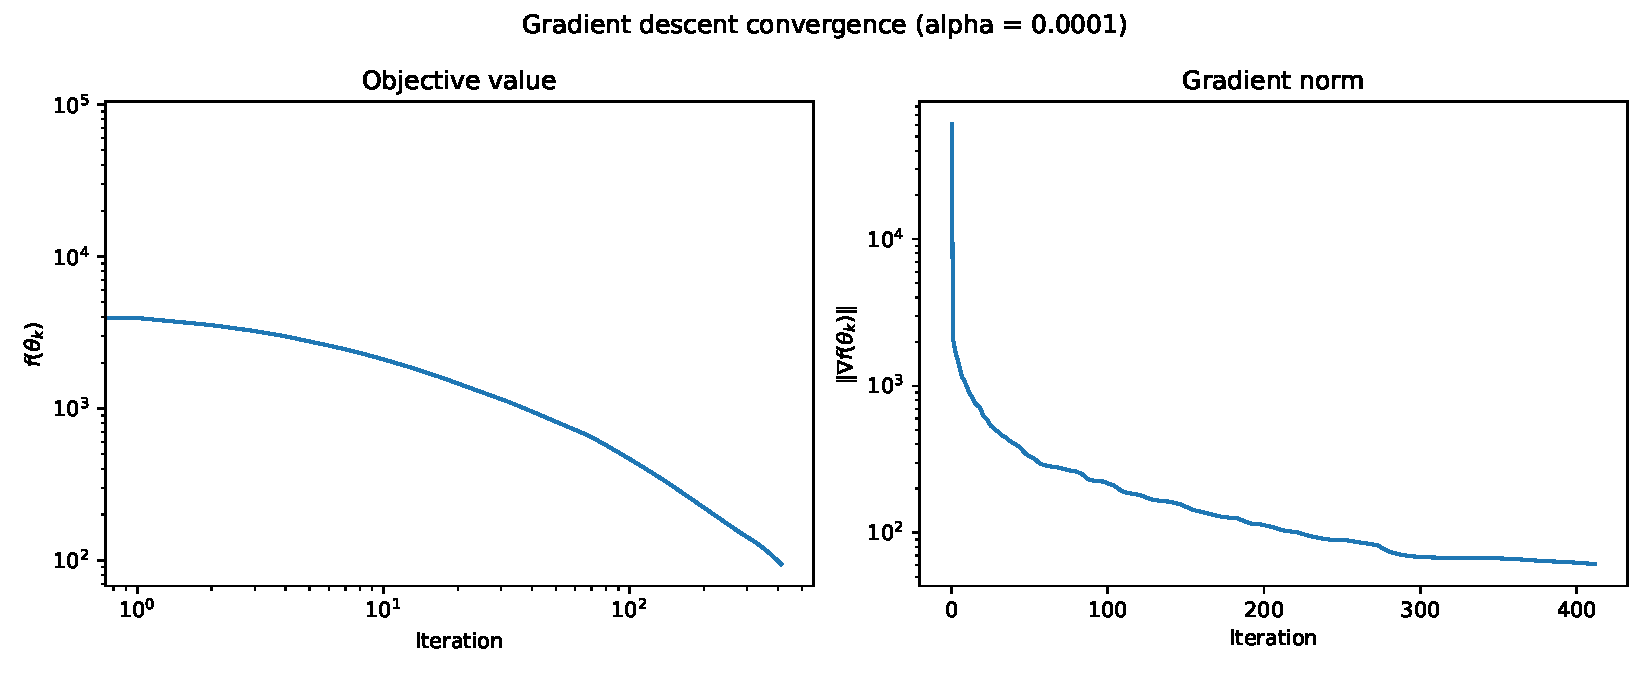
\includegraphics[width=0.9\linewidth]{results/q5_convergence.pdf}
    \caption{Convergence of fixed-step gradient descent with $\alpha=10^{-4}$. The objective value and gradient norm are shown as functions of the iteration number.}
    \label{fig:q5_convergence}
\end{figure}

We use a linear horizontal axis for the iteration number and logarithmic vertical axes for both quantities. This choice is appropriate because both $f_\lambda(\theta_k)$ and $\norm{\nabla f_\lambda(\theta_k)}$ decrease over several orders of magnitude, which is displayed more clearly on a logarithmic scale.

At the initial point, the objective value is $f_\lambda(\theta_0)=14144.6160$ and the gradient norm is $\norm{\nabla f_\lambda(\theta_0)}=16492.0716$. The method stops after $1546$ iterations with $f_\lambda(\theta_{1546})=5.61665$ and $\norm{\nabla f_\lambda(\theta_{1546})}=16.4697$. Based on these values, we confirm the run terminates due to the gradient tolerance rather than the time limit.

\section*{Question 6}

The strongest applicable result is Theorem 4.31 of the lecture notes, with Corollary 4.32. If $f$ is $\mu$-strongly convex with $L$-Lipschitz gradient, GD with step $1/L$ satisfies $f(\theta_k) - f(\theta^*) \le (1 - 1/\kappa)^k\,(f(\theta_0) - f(\theta^*))$, where $\kappa = L/\mu$. Moreover, $\theta_k \to \theta^*$ and $\nabla f(\theta_k) \to 0$, all at least linearly.

The assumptions hold. By Question 1, $f_\lambda$ is differentiable and $\lambda$-strongly convex ($\mu = \lambda$) with a unique minimizer $\theta^*$. By the assignment, $\nabla f_\lambda$ is $L$-Lipschitz with $L = \sigma_{\max}(X)^2 + \lambda = 7.94\cdot 10^5$, where $X = [\tilde x_1, \dots, \tilde x_m]$; hence $\kappa = 1.59\cdot 10^8$.

Any $L' \ge L$ is also a Lipschitz constant. Taking $L' = 1/\alpha$, the theorem therefore applies to every $\alpha \in (0, 1/L] = (0, 1.26\cdot 10^{-6}]$, with rate $1 - \alpha\lambda$. Our $\alpha = 10^{-4}$ ($\alpha L \approx 79$) is not covered; of our grid, only $10^{-6}$ and $10^{-7}$ are. \\ The local Theorem 3.15 requires $C^2$, which fails here because $\phi''$ jumps at $-1$ and $0$.

\paragraph{Comparison.} The theory predicts monotone decrease (Theorem 3.4) and linear convergence, but at rate $1 - 1/\kappa \approx 1 - 6\cdot 10^{-9}$. Over 1546 iterations this guarantees essentially nothing, and the covered step sizes indeed progress very slowly (see Question 4).

Our run does much better: $f_\lambda$ and $\|\nabla f_\lambda\|$ decrease monotonically, and $f_\lambda$ drops by a factor above $2500$ (Figure 2). This happens even though our step is about $79$ times larger than $1/L$, which is consistent with the remark following Definition 3.1: (3.1) only needs to hold in the regions the algorithm explores, whereas $L$ is a bound valid on all of $\mathcal E$, determined by $X$ only through $\sigma_{\max}(X)$; on the region our iterates actually visit, a smaller constant may suffice.

Finally, the run stopped on the gradient tolerance with $\|\nabla f_\lambda\| = 16.5$. Combining (4.5) and (4.7) gives $\|\theta - \theta^*\| \le \|\nabla f_\lambda(\theta)\|/\mu \approx 3.3\cdot 10^{3}$, so with $\mu = \lambda$ this small, the stopping point is not certified to be close to $\theta^*$: the finite run shows the early behaviour, not the limit described by Theorem 4.31.


\section*{Question 7}
Using the final iterate $\theta_{\mathrm{final}}$ from Question 5, we predicted label $1$ whenever $\widetilde{x}_i^{\mathsf{T}}\theta_{\mathrm{final}}>0$ and label $0$ otherwise. On the training set, the classifier made $2$ incorrect predictions out of $12665$ samples, resulting in an error rate of
\[
\frac{2}{12665} \approx 0.0001579 \quad (0.0158\%).
\]
On the test set, it made $3$ incorrect predictions out of $2115$ samples, resulting in an error rate of
\[
\frac{3}{2115} \approx 0.0014184 \quad (0.1418\%).
\]
The test error is slightly higher than the training error, but both error rates are very small. This suggests that the classifier generalizes well to unseen data, with little evidence of substantial overfitting. However, a more reliable conclusion would require testing multiple regularization parameters and, ideally, using cross-validation or a separate validation set. Since the test set contains only three errors, the observed difference between training and test performance should also be interpreted with some caution.

\section*{Question 8}
Through this homework, we practiced calculating the gradient of a function using the definition of differential, as opposed to coordinate-based methods such as partial derivatives. We deployed at our advantage the basic properties of the differential, such that it is linear and that it acts identically on linear maps (i.e. $\D f(x)[v]=L(v)$, for any linear map $L$).

We also verified how strongly-convex maps are ideal for optimization problems, since they have exactly one minimizer (global and local), which coincides with the only critical point (cf. Question 1). If the objective function is, moreover, Lipschitz, gradient descent gives an algorithmic way of finding such a minimizer.

On the computational side, we learned how vectorization of the code reduces run-time. We also observed that computational checks, although useful for detecting errors, do not constitute a proof of correctness, repeating experiments and comparing numerical statistics can nevertheless provide stronger evidence.

Floating-point effects must also be taken into account when interpreting numerical results. In particular, catastrophic cancellation and finite-precision arithmetic can cause practical computations to deviate from their exact theoretical behavior, as observed in Question 3.

Furthermore, step sizes that perform well in practice may differ substantially from conservative values used in theoretical sufficient conditions. Such guarantees are designed to hold generally and may not exploit the particular structure of the data. For image data, for example, correlations between pixels could potentially be exploited through dimensionality reduction, although unsupervised methods such as PCA may discard directions that are important for discriminating between the two classes.

Finally, it is important to distinguish training data from validation or test data in order to assess whether the obtained solution generalizes to unseen samples.

\end{document}


